\chapter{Repository structure}
\section{Repository folder structure}

The repository is divided into folders that correspond to the function of the files within it. Figure \ref{fig:repo_folder_diagram} shows how the repository is structured.


\begin{figure}[h]
    \centering
    \includesvg[width=0.8\textwidth]{repo_folders.svg}
    \caption{Repository structure}
    \label{fig:repo_folder_diagram}
\end{figure}




\section{Python tools}

\subsection{Filter class}

For this project, a filter class was written in Python to simulate the behaviour of a hardware filter. The filter class also includes methods to process the incoming data such as convolution.

\lstinputlisting[language=Python, caption=FIR filter class methods, label=fir_filter_class]{listings/fir_class.py}


\subsection{GUI viewer}

The image viewer is a helpful tool to visualize the processed data from the camera sensor. Figure \ref{fig:image_viewer_scr_1} is a screenshot of the image viewer and its structure.


\begin{figure}[h]
    \centering
    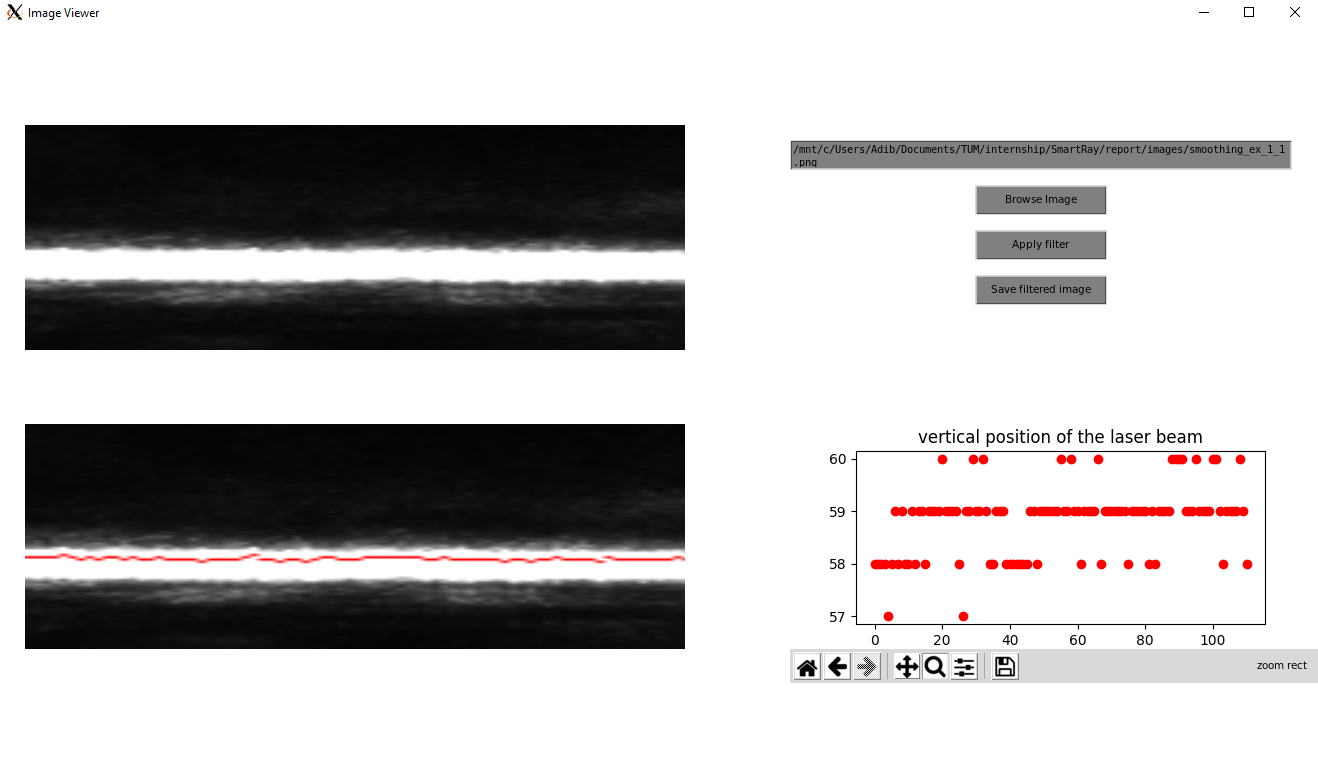
\includegraphics[width=0.8\textwidth]{image_viewer_scr_1.png}
    \caption{Image viewer tool}
    \label{fig:image_viewer_scr_1}
\end{figure}

The viewer is built using Python and TKinter with TkAgg as a rendering backend. The program is built using a mixture of OOP and functional programming paradigms. This is because of how TKinter widgets interact with each other.

Image viewer accepts only grayscale images as shown in Figure \ref{fig:image_viewer_scr_1}. In addition, the Image Viewer has slow processing time for large images because the processing is done sequentially, as concurrency isn't really optimal in Python since it doesn't provide significant speedup.


\subsection{VHDL test vector generation scripts}
\emergencystretch 4em%
    {\sloppy
        Two scripts were written to assist in executing VHDL testbenches. \lstinline{test_vector_file_gen.py} \& \lstinline{test_vector_file_data_viewer.py} are the scripts in the repository. \lstinline{test_vector_file_gen} reads image data from the \lstinline{misc} folder and exports a \lstinline{.txt} file with the correct fomatting for the \lstinline{CTRL} and \lstinline{DATA} signals. Those two signals are the inputs of the system, \lstinline{CTRL} is a 2-bit control signal (see Table \ref{tab:ctrl_table}) and \lstinline{DATA} is an 8-bit pixel value.
}

\section{VHDL code and hardware implementation}

VHDL modules within the repository are divided into their functional behaviour. Development of the VHDL system modules followed a structural design pattern, thus all of the basic digital components has been written in VHDL to ensure consistency in behaviour and avoid synthesizer ambiguity. In this section, only the major system modules will be explained. The rest are shown in Appendix A.

\subsection{FIR filter}
FIR filters are generally easy to implement in VHDL as they are only composed of multipliers, adders and basic registers. On the other hand, the decision of which architecture to implement comes with tradeoffs that depend on the general goal of the filter design. Figure \ref{fig:fir_filter_architectures} shows 4 possible filter architectures Direct FIR, Transposed FIR, pipelined Transposed FIR and Folded Direct FIR filters \cite{Akif1256720}.


\begin{figure}[h]
    \centering
    \includesvg[width=0.5\textwidth]{fir_architecture.svg}
    \caption{(a) Direct FIR, (b) Transposed FIR, (c) Pipelined Transposed FIR, (d) Folded Direct FIR}
    \label{fig:fir_filter_architectures}
\end{figure}

Direct FIR filter is the basic version of FIR filters, it is what would be basically seen in a DSP hard IP core. There is a major design shortcoming which is a very long combinational critical path from the multipliers to the output through adders as shown in Figure \ref{fig:direct_fir_filter_architectures_crit_path}


\begin{figure}[h]
    \centering
    \includesvg[width=1\textwidth]{direct_fir_filter_delay.svg}
    \caption{Critical path in Direct FIR architecture}
    \label{fig:direct_fir_filter_architectures_crit_path}
\end{figure}

The critical path delay as shown in \eqref{direct_fir_crit_path} highlights the problem with the Direct FIR design. Where $N$ is the size of the filter.


\begin{equation}\label{direct_fir_crit_path}
    \begin{aligned}
        T_{crit} = T_{mul} + (N-1) * T_{adder}
    \end{aligned}
\end{equation}

On the other hand, the Transposed FIR filter design breaks down the critical path as shown in Figure \ref{fig:transposed_fir_filter_architectures_crit_path}. The critical path delay is $T_{crit} = T_{mul} + T_{adder}$


\begin{figure}[h]
    \centering
    \includesvg[width=1\textwidth]{transposed_fir_filter_delay.svg}
    \caption{Critical path in Transposed FIR architecture}
    \label{fig:transposed_fir_filter_architectures_crit_path}
\end{figure}


The pipelined transposed FIR architecture breaks down the critical path further into being $T_{mul}$ but introduces $2*N$ more registers, where $N$ is the filter size. Also, a bigger fanout is introduced to the $X[n]$ signal as well. The introduced trade-off in the design area is a decision that has to be made. During this project, the transposed FIR filter architecture was the one implemented.

The VHDL implementation was done using generate statements which take into account the filter generic. Figure \ref{fig:fir_filter_hdl_specs} shows extensive details about the module implementation in VHDL. The data was generated using TerosHDL in vscode.


\begin{figure}[h]
    \centering
    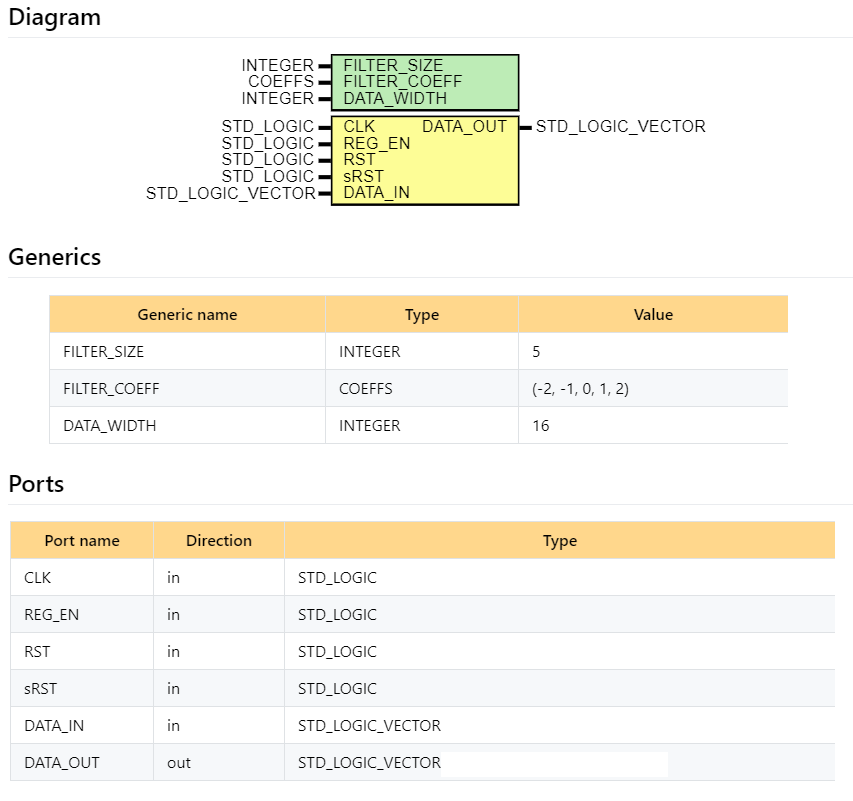
\includegraphics[width=0.8\textwidth]{fir_filter_hdl_specs.png}
    \caption{FIR filter HDL specs}
    \label{fig:fir_filter_hdl_specs}
\end{figure}

As shown in Figure \ref{fig:fir_filter_hdl_specs}, the filter coefficients, filter size and the input/output data width are generics which can be specified at module instantiation.

\subsection{Zero crossing module}

The zero-crossing algorithm is fairly simple and straight-forward to implement, since the implementation of the algorithm depends on the module finding the maximum and minimum values in the pixel column. Therefore, a peak-detector module was written in VHDL. The peak-detector clocks out the index of the peak value whether it was a maximum or a minimum peak.

After the indicies of both peaks has been acquired, another module ensures that the index of the maximum value is less than the index of the minimum value, because we are looking for a positive to negative going zero crossing. The module ensures that by clocking out both indicies if the values are correct, otherwise it clocks out zeros.

Finally, the zero crossing index is calculated according to \eqref{zero_index_eq}. The zero index is then clocked out of the module. Figure \ref{fig:zero_crossing_final} shows the structure of the zero-crossing module. The abundant registers are there for delay matching.


\begin{figure}[h]
    \centering
    \includesvg[width=1\textwidth]{zero_crossing_final.svg}
    \caption{Zero-crossing structural view}
    \label{fig:zero_crossing_final}
\end{figure}

Figure \ref{fig:zero_crossing_hdl_specs} shows the specifications of the zero crossing module.


\begin{figure}[h]
    \centering
    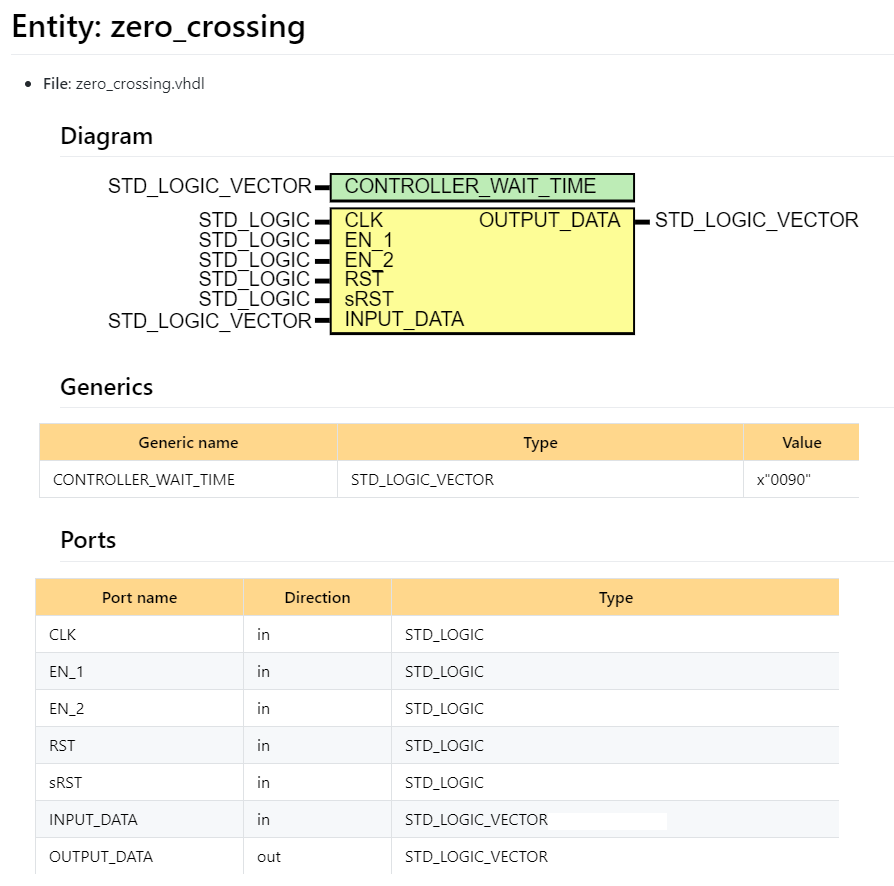
\includegraphics[width=0.6\textwidth]{zero_crossing_hdl_specs.png}
    \caption{Zero-crossing HDL specs}
    \label{fig:zero_crossing_hdl_specs}
\end{figure}

\subsection{Input controller}

The last part of the 3 major system modules is the input controller. The input controller takes the 8-bit pixel data and converts it to 16 bit. It also takes two control bits which specify the type of the data it is receiving. Table \ref{tab:ctrl_table} shows what each \texttt{CTRL} value corresponds to in terms of package type.

\begin{table}[h]
    \centering
    \begin{tabular}{ l | c }
        CTRL & TYPE  \\
        \hline \hline
        0b00 & IDLE  \\
        0b01 & START \\
        0b10 & DATA  \\
        0b11 & STOP  \\
    \end{tabular}
    \caption{Input controller control bits}
    \label{tab:ctrl_table}
\end{table}


The input controller is basically a state machine with the enable and reset signals of the system modules as its outputs. Figure \ref{fig:input_controller_hdl_specs} shows the specifications of the input controller. The module also has generics that control the timings of the output pins, the enable outputs go logic '0' when the module is flushed out of useful data.


\begin{figure}[h]
    \centering
    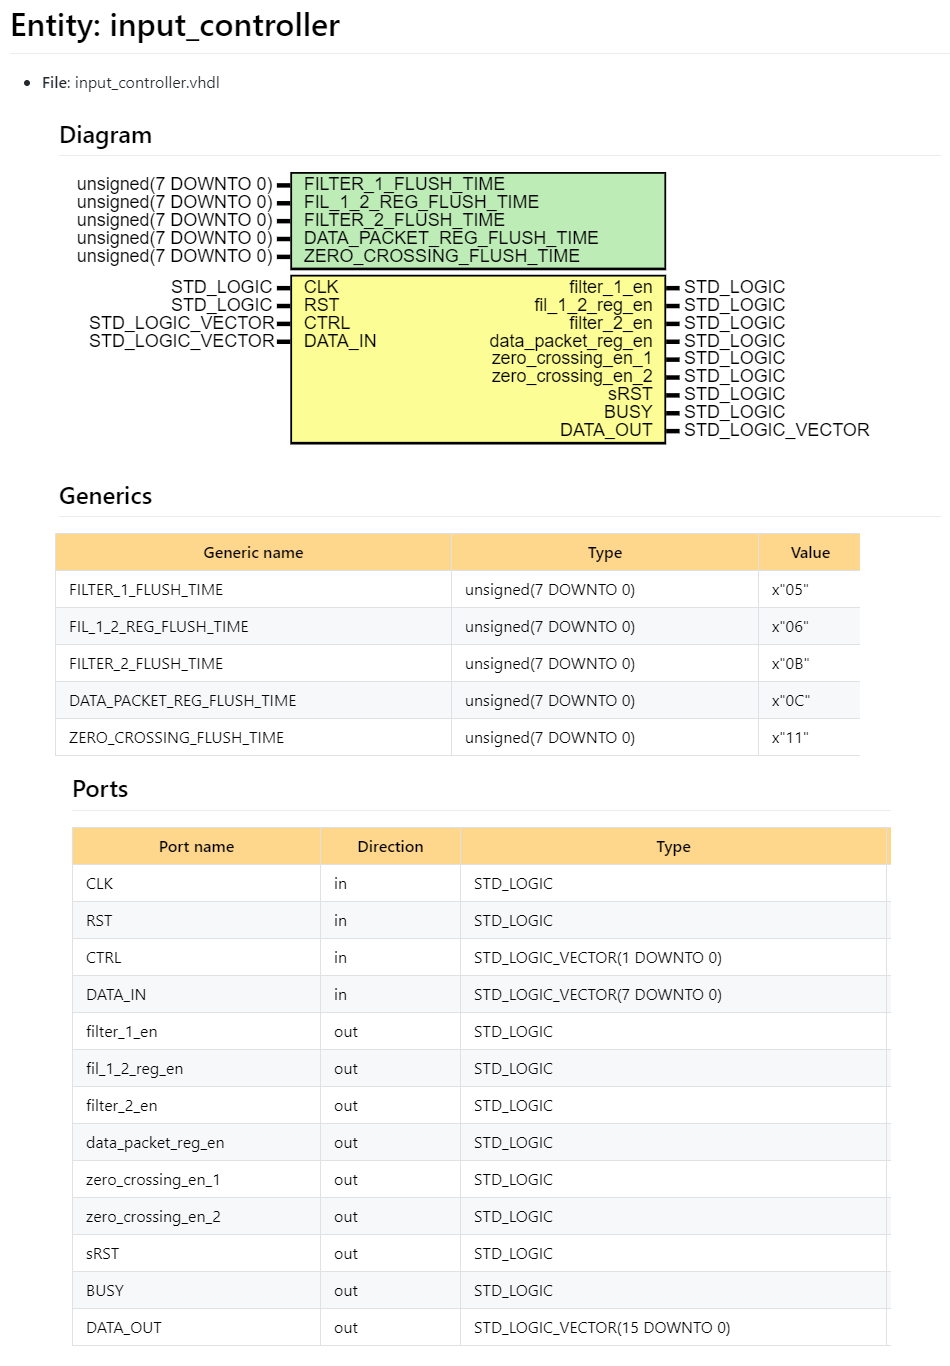
\includegraphics[width=0.8\textwidth]{input_controller_hdl_specs.png}
    \caption{Input controller HDL specs}
    \label{fig:input_controller_hdl_specs}
\end{figure}


The state machine depends on an internal counter that counts the clock cycles. Figure \ref{fig:input_controller_state_machine} shows the state diagram of the input controller's state machine.



\begin{figure}[h]
    \centering
    \includesvg[width=0.8\textwidth]{input_controller_state_machine.svg}
    \caption{Input controller state machine}
    \label{fig:input_controller_state_machine}
\end{figure}


During the \texttt{STOPPING} state, there are several conditions to check against the internal counter to disable the modules sequentially depending on the time it takes to flush those modules out.


\subsection{TOP module}

The TOP module is just a structural combination of all the aforementioned sub-system modules. Figure \ref{fig:final_sys_overview} shows the block diagram of the system. The index counter module is basically a counter that starts counting after a specified delay. This module is used to combine the delayed output data from the filters with their indicies so they can be used in the zero crossing module.


\begin{figure}[h]
    \centering
    \includesvg[width=0.8\textwidth]{final_sys_overview.svg}
    \caption{Block diagram of TOP}
    \label{fig:final_sys_overview}
\end{figure}

\section{Build system}

The VHDL code analysis, elaboration and simulation are all done using GHDL. The main appeal of the tool is the ability of working with VHDL modules from the terminal. GHDL allows the user to generate a wave \texttt{.vcd} file, the wave file can be viewed using GTKWave.

To automate the process of code analysis, elaboration, and simulation Make was used. The MakeFile is located in the build folder in the repository where all the compiled binaries are located as well. The MakeFile also provides some other functionality to the user such as viewing the wavefiles in GTKWave.

